\documentclass[relatorio.tex]{subfiles}
\begin{document}
Para o desenvolvimento deste projeto, foi utilizada uma estratégia de programação
orientada aos modelos, i.e. foi desenvolvido a maioria dos diagramas de sequência
e de classe, posteriormente procedeu-se à implementação do código.

Esta estratégia permitiu que se antecipasse bastantes problemas de métodos
(assinaturas, valores retornados), assim como identificar classes de implementação necessárias.
Apesar disso, ao longo da implementação denotou-se ainda algumas falhas que obrigaram a alterações pontuais.

No entanto, fruto da estratégia utilizada a implementação do código foi realizada em aproximadamente
2/ 3 dias, conforme distribuído através de um diagrama de Gantt (ver \ref{img:diagrama_gantt}).

Para facilitar o trabalho em grupo, utilizou-se um repositório no \textit{GitHub} para efetuar
\textit{source control} e o programa \textit{Visual Paradigm} com a funcionalidade de \textit{Team} e
\textit{Tasifier}.
Este último, revelou-se fundamental, pois permitiu a distribuição das tarefas pelos elementos
e o feedback sobre o mesmo.

Ao nível de código, utilizou-se um projeto \textit{Maven} para gerir os \textit{imports} necessários,
principalmente ao nível de testes. Infelizmente, não foi possível desenvolver testes suficientes
devido à falta de tempo, ficando pendente os testes relacionados com o \underline{GestReparacoesFacade}.

\begin{landscape}
    \begin{figure} [!ht]
        \centering
        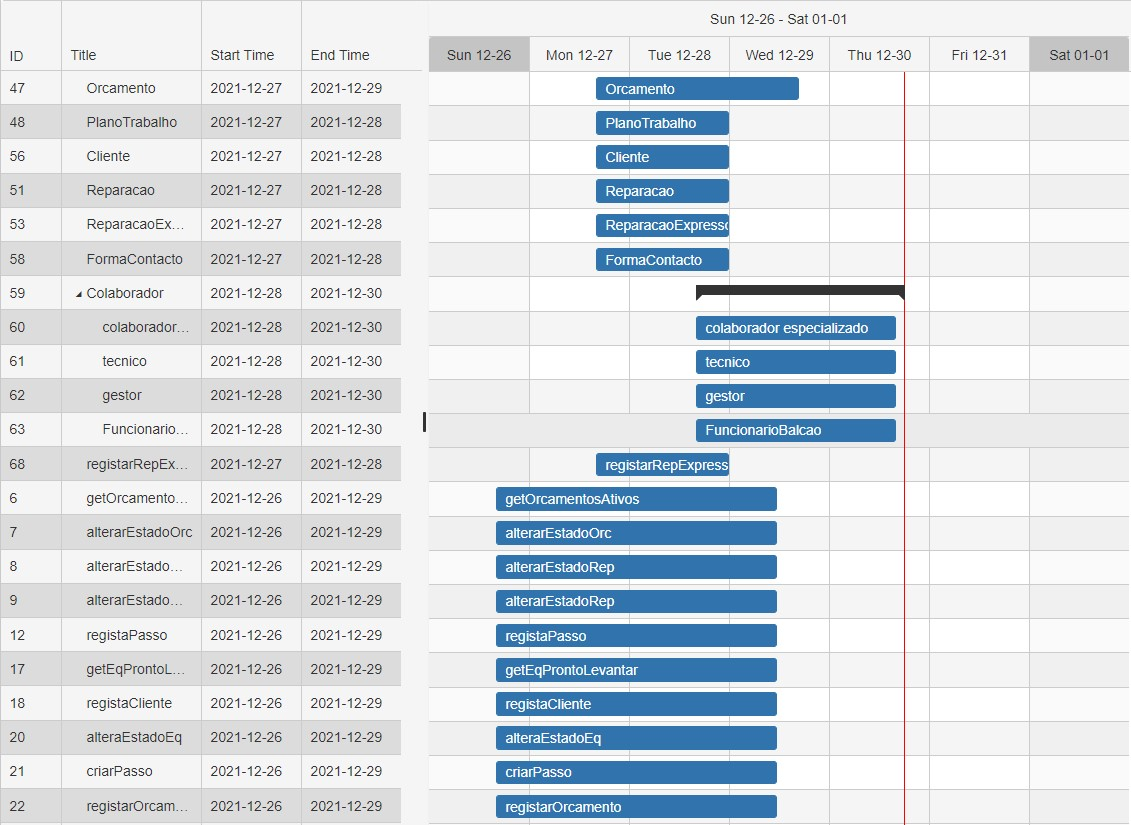
\includegraphics[width=\linewidth]{gantt.jpg}
        \caption{Recorte do diagrama de Gantt} \label{img:diagrama_gantt}
    \end{figure}
\end{landscape}

\section{Menus}

Os menus foram desenhados de maneira a corresponder a todas as funcionalidades descritas nos \textit{Use Cases}.

\begin{figure}[!ht]
    \centering
    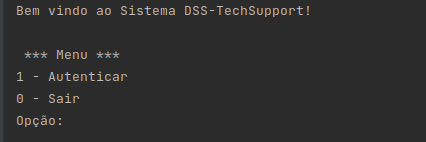
\includegraphics[scale=0.60]{MenuInicial.png}
    \caption{Menu inicial}
\end{figure}

\begin{figure}[!ht]
    \centering
    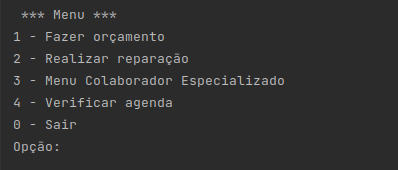
\includegraphics[scale=0.60]{MenuTecnico.png}
    \caption{Menu Técnico}
\end{figure}

\begin{figure}[!ht]
    \centering
    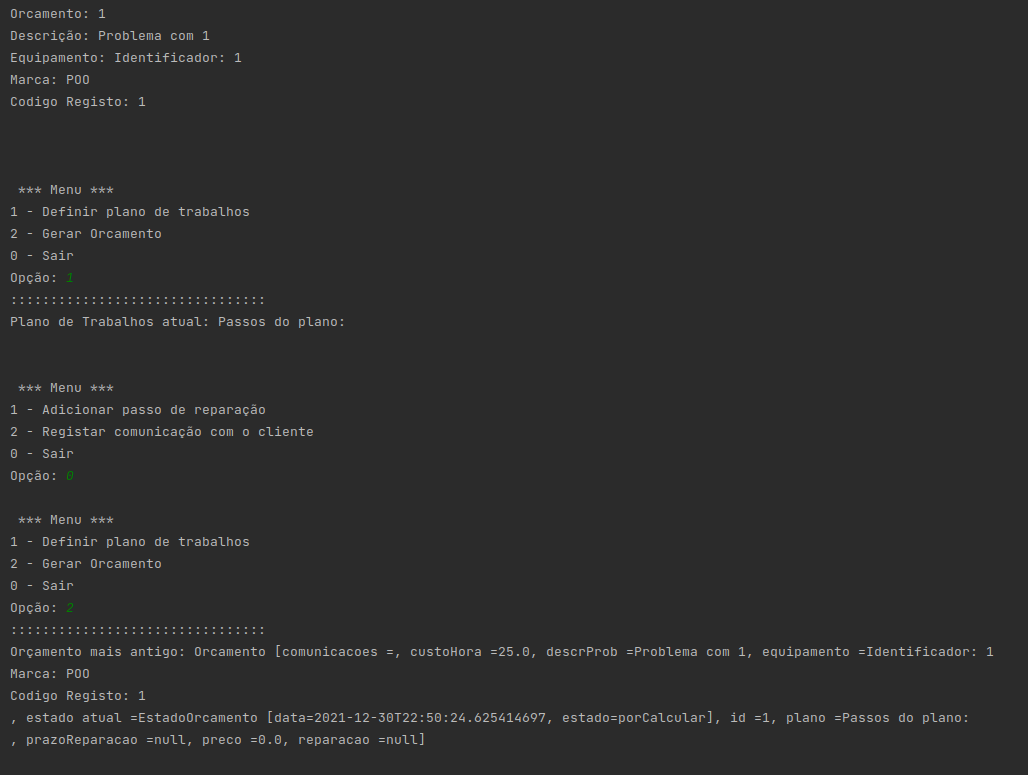
\includegraphics[scale=0.30]{fazerOrcamento.png}
    \caption{Menu Fazer orcamento}
\end{figure}

\begin{figure}[!ht]
    \centering
    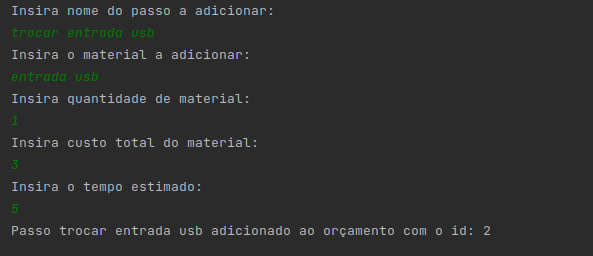
\includegraphics[scale=0.60]{adicionarPasso.png}
    \caption{Exemplo Adicionar Passo}
\end{figure}


\begin{figure}[!ht]
    \centering
    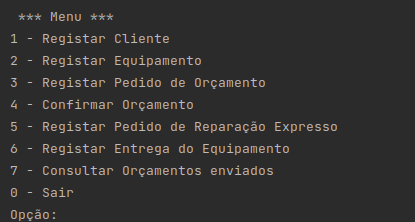
\includegraphics[scale=0.60]{MenuFuncBalcao.png}
    \caption{Menu Funcionário Balcão}
\end{figure}

\begin{figure}[!ht]
    \centering
    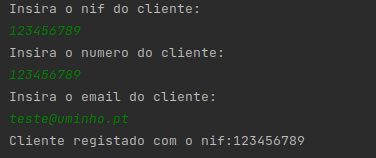
\includegraphics[scale=0.60]{registarCliente.png}
    \caption{Exemplo registar cliente}
\end{figure}

\begin{figure}[!ht]
    \centering
    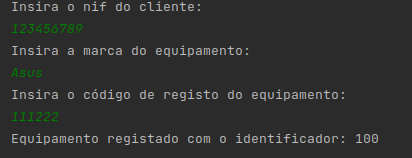
\includegraphics[scale=0.60]{registarEquipamento.png}
    \caption{Exemplo registar equipamento}
\end{figure}

\begin{figure}[!ht]
    \centering
    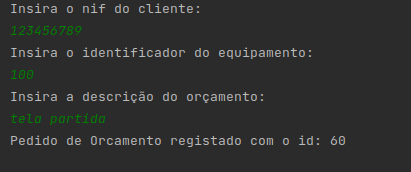
\includegraphics[scale=0.60]{RegistarPedOrc.png}
    \caption{Exemplo pedir orcamento}
\end{figure}

\begin{figure}[!ht]
    \centering
    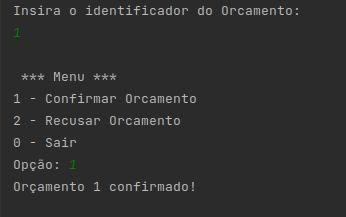
\includegraphics[scale=0.60]{ConfirmarOrc.png}
    \caption{Exemplo confirmar orcamento}
\end{figure}

\begin{figure}[!ht]
    \centering
    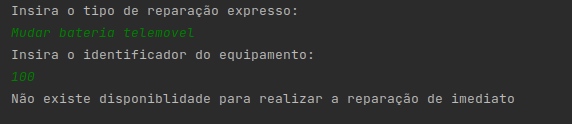
\includegraphics[scale=0.60]{pedidoRepExpresso.png}
    \caption{Exemplo pedir reparação expresso}
\end{figure}

\begin{figure}[!ht]
    \centering
    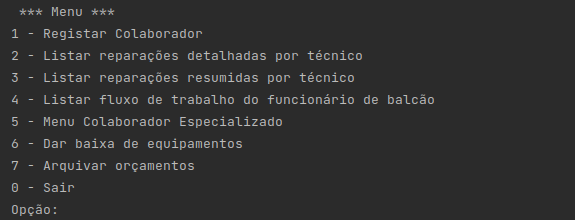
\includegraphics[scale=0.60]{MenuGestor.png}
    \caption{Menu Gestor}
\end{figure}

\end{document}